\chapter{Numerical Experiments} \label{chap:numerical-experiments}
In this chapter, we will solve the polynomial eigenvalue problem, Eq.~(\ref{eq:polynomial-eigenvalue-problem}), under different boundary conditions.

For subsonic and supersonic velocity profiles, spectral methods will be used. More specifically, spectral-collocation and spectral-Galerkin methods are employed. Eq.~(\ref{eq:polynomial-eigenvalue-problem}) will be solved under Dirichlet boundary condition and fixed-open boundary condition. The former boundary condition indicates that the perturbation is 0 at the nozzle entrance and exit $\tilde{v}(\pm 1)=0$. The fixed-open boundary condition means $\tilde{v}(-1)=\tilde{v}'(1) = 0$. By comparing the results from two spectral methods, we ensure the accuracy and reliability of the results. The parameters of spectral method are summarized in Table.~(\ref{table:parameters}). For spectral-collocation method, we use 101 points, and for spectral-Galerkin method we use 101 points and 30 basis functions.

\begin{table} [htbp]
	\centering
	\caption{With Dirichlet boundary condition, all methods have good accuracy, so using 101 nodes in the region $[0,1]$ is enough. For FE and SE methods, we use 50 basis functions.}
	\begin{tabular}{|c|c|c|}
		\hline
		                              & Collocation & Galerkin \\
		\hline
		M (number of points)          & 101         & 101      \\
		\hline
		N (number of basis functions) &             & 30       \\
		\hline
	\end{tabular}
	\label{table:parameters}
\end{table}

When dealing with accelerating and decelerating velocity profiles, as outlined in Chap.~\ref{chap:singular-perturbation}, the spectral method struggles to yield meaningful results because of the singularity at the nozzle throat ($z=0$). In such cases, we will resort to the shooting method for resolution. We will set boundary condition to $\tilde{v}(-1) = 0$ and $\tilde{v}(0)=1$.

\section{Subsonic Case}
\subsection{Constant Velocity Profile}
Eq.~(\ref{eq:constant-v-problem-dirichlet}) is a special case of a more general polynomial problem Eq.~(\ref{eq:polynomial-eigenvalue-problem}). The existence of the exact solution allows us to verify the correctness of each method's implementation. This also serves as a reference to the accuracy spectral methods can achieve.

\subsubsection*{Dirichlet Boundary}
Fig.~\ref{fig:constant-subsonic-dirichlet} shows that the eigenvalues obtained by spectral methods agree with the theoretical eigenvalues. Table.~\ref{table:eigenvalue-error-constant-subsonic-dirichlet} shows us the relative error $\abs{\omega_{numeric} - \omega_{analytic}}/\abs{\omega_{analytic}}$ is about $~10^{-14}$. Spectral methods indeed have high accuracy.

\begin{table} [H]
	\centering
	\caption{Relative errors of first 5 eigenvalues obtained by spectral methods in constant subsonic velocity case with Dirichlet boundary condition. Numerical results agree with exact solution well.}
	\begin{tabular}{|c|c|c|c|c|c|}
		\hline
		$v_0=0.5$   & $\omega_1$     & $\omega_2$     & $\omega_3$     & $\omega_4$     & $\omega_5$     \\
		\hline
		Collocation & 3.48944421e-14 & 6.72512513e-14 & 1.59603736e-14 & 9.81718764e-15 & 4.07098462e-15 \\
		\hline
		Galerkin    & 4.09596742e-14 & 1.65697986e-14 & 4.97650778e-14 & 3.27344763e-13 & 4.11444935e-12 \\
		\hline
	\end{tabular}
	\label{table:eigenvalue-error-constant-subsonic-dirichlet}
\end{table}

\begin{figure}[H]
	\centering
	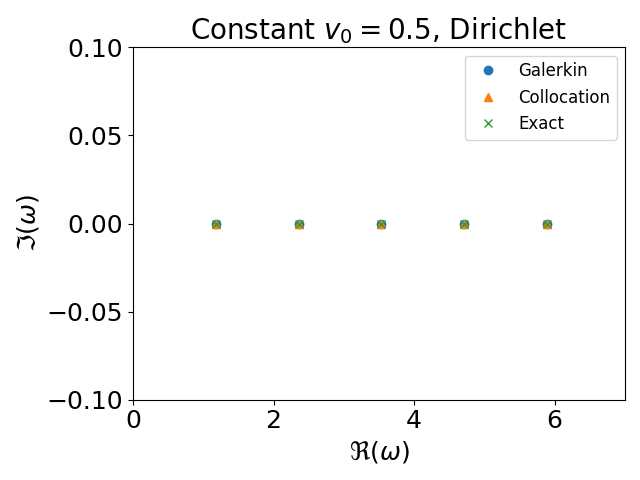
\includegraphics[width=0.7\linewidth]{figures/constant-subsonic-dirichlet.png}
	\caption{Showing the first 5 eigenvalues of each method. They are stable. Spectral methods agree with exact eigenvalues.}
	\label{fig:constant-subsonic-dirichlet}
\end{figure}


\subsubsection*{Fixed-Open Boundary}
The numerical eigenvalues agree with the exact eigenvalues. The relative errors $\abs{\omega_{numeric} -\omega_{analytic}}/\abs{\omega_{analytic}}$ are about $10^{-13}$. Again spectral methods has good accuracy.
\begin{table} [H]
	\centering
	\caption{Relative error of each eigenvalue. Notice that the mode index starts from 0. These results agree with theory.}
	\begin{tabular}{|c|c|c|c|c|c|}
		\hline
		$v_0=0.5$   & $\omega_0$     & $\omega_1$     & $\omega_2$     & $\omega_3$     & $\omega_4$     \\
		\hline
		Collocation & 2.36006260e-12 & 1.95269435e-13 & 6.78183927e-14 & 2.43078107e-14 & 4.17011610e-14 \\
		\hline
		Galerkin    & 2.52491323e-12 & 2.19414097e-13 & 1.82417919e-13 & 5.92948284e-13 & 4.41481039e-12 \\
		\hline
	\end{tabular}
	\label{table:eigenvalue-error-fixed-open-subsonic}
\end{table}

\begin{figure}[H]
	\centering
	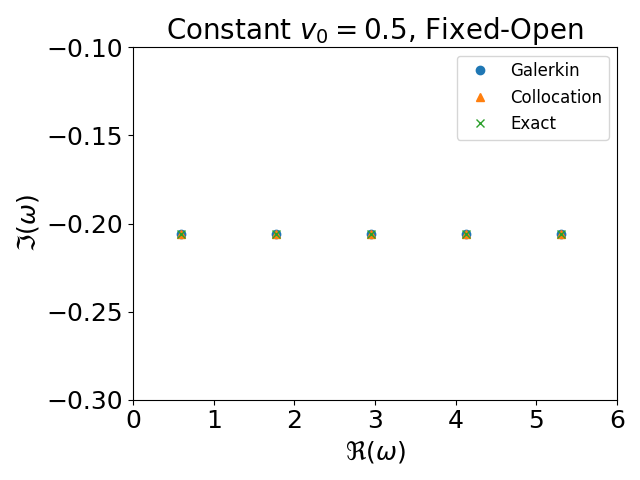
\includegraphics[width=0.7\linewidth]{figures/constant-subsonic-fixed-open.png}
	\caption{Showing the first 5 eigenvalues of each method. They are stable. The spectral methods agree with the exact eigenvalues.}
	\label{fig:constant-subsoniv-fixed-open}
\end{figure}


\subsection{Variable Velocity Profile}
\subsubsection*{Dirichlet Boundary}
When setting the mid-point velocity to be $M_m=0.5$, we have the subsonic velocity profile. This velocity profile is the orange line shown in Fig.~\ref{fig:velocity-profiles}. With Dirichlet boundary condition, $\tilde{v}(\pm 1) =0$. The flow in magnetic nozzle is stable. Fig.~\ref{fig:subsonic-dirichlet} shows the first few eigenvalues obtained by different discretizations.

The order of growth rates obtained by different methods is $10^{-13}$, we can consider it to be stable.
\begin{figure} [H]
	\centering
	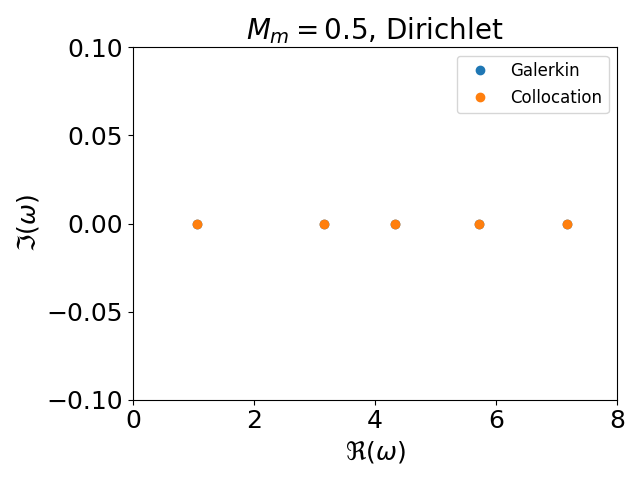
\includegraphics[width=0.7\linewidth]{figures/subsonic-drichlet.png}
	\caption{Showing the first 5 modes. They are stable. Two methods agree with each other.}
	\label{fig:subsonic-dirichlet}
\end{figure}

\subsubsection*{Fixed-Open Boundary}
\begin{figure} [H]
	\centering
	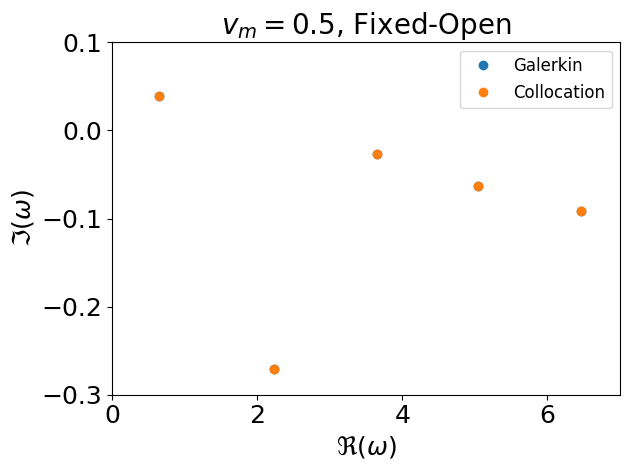
\includegraphics[width=0.7\linewidth]{figures/subsonic-fixed-open.png}
	\caption{Showing the first 5 modes. The ground mode is unstable, other modes are stable.}
	\label{fig:subsonic-fixed-open}
\end{figure}


\section{Supersonic Case}
\subsection{Constant Velocity Profile}
\subsubsection*{Dirichlet Boundary}
Table.~\ref{table:eigenvalue-error-dirichlet-supersonic} shows good agreement between the spectral methods and the theoretical eigenvalues. However, we see that the accuracy of spectral-Galerkin method drops for larger eigenvalues.
\begin{table} [H]
	\centering
	\caption{Relative error of each eigenvalue. Numerical results agree with the theory, but we see the accuracy of eigenvalues obtained from spectral-Galerkin method drops after the 3rd one.}
	\begin{tabular}{|c|c|c|c|c|c|}
		\hline
		$v_0=1.5$   & $\omega_1$     & $\omega_2$     & $\omega_3$     & $\omega_4$     & $\omega_5$     \\
		\hline
		Collocation & 2.08984845e-13 & 9.29501612e-14 & 4.24537846e-14 & 3.38103217e-14 & 1.74476052e-14 \\
		\hline
		Galerkin    & 1.64805562e-13 & 6.09485884e-14 & 6.81795167e-12 & 1.95656738e-09 & 1.54134402e-07 \\
		\hline
	\end{tabular}
	\label{table:eigenvalue-error-dirichlet-supersonic}
\end{table}

\begin{figure}[H]
	\centering
	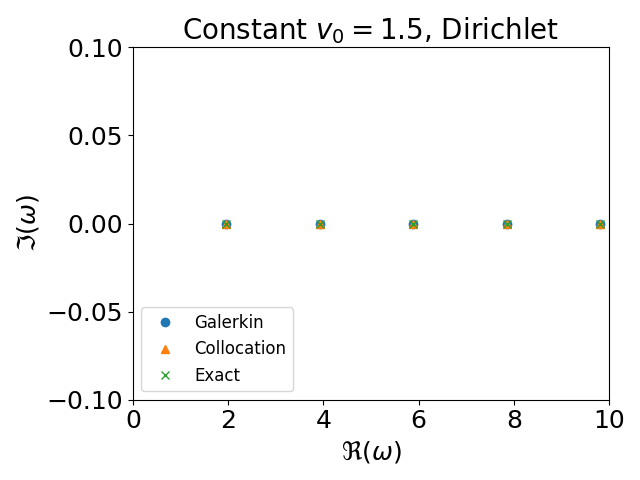
\includegraphics[width=0.7\linewidth]{figures/constant-supersonic-dirichlet.png}
	\caption{Showing the first 5 eigenvalues of each method. They are stable. All methods agree with the exact eigenvalues.}
	\label{fig:constant-supersonic-dirichlet}
\end{figure}

\subsubsection*{Fixed-Open Boundary}
From Table.~\ref{table:eigenvalue-error-fixed-open-supersonic} we see that the accuracy of spectral-Galerkin method drops for larger eigenvalues.
\begin{table} [H]
	\centering
	\caption{Relative error of eigenvalue obtained by spectral methods in constant supersonic case under fixed-open boundary. Results agree with theory. The accuracy of spectral-Galerkin method drops after first few eigenvalues.}
	\begin{tabular}{|c|c|c|c|c|c|}
		\hline
		$v_0=1.5$   & $\omega_0$     & $\omega_1$     & $\omega_2$     & $\omega_3$     & $\omega_4$     \\
		\hline
		Collocation & 5.10516649e-11 & 3.58709292e-12 & 8.72529437e-13 & 3.24263319e-13 & 1.34297439e-13 \\
		\hline
		Galerkin    & 5.38682371e-11 & 4.31902441e-12 & 1.44799870e-12 & 8.02395621e-11 & 2.05280524e-09 \\
		\hline
	\end{tabular}
	\label{table:eigenvalue-error-fixed-open-supersonic}
\end{table}

\begin{figure}[H]
	\centering
	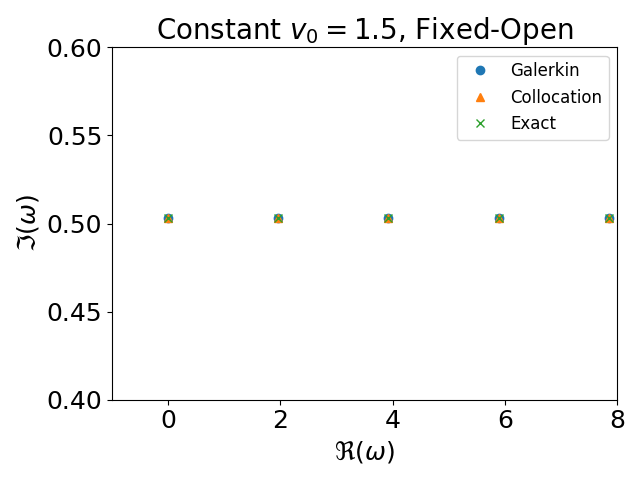
\includegraphics[width=0.7\linewidth]{figures/constant-supersonic-fixed-open.png}
	\caption{Showing the first 5 filtered eigenmodes of each method. They are unstable. The spectral methods agree with theoretical eigenvalues.}
	\label{fig:constant-supersonic-fixed-open}
\end{figure}

\subsection{Variable Velocity Profile}
\subsubsection*{Dirichlet Boundary}
When the velocity profile is supersonic, shown as purple line in Fig.~\ref{fig:velocity-profiles}, spurious modes appeared as predicted in Chap.~\ref{chap:theoretical-analysis}. Using the convergence test, we successfully eliminate all unstable modes. Fig.~\ref{fig:supersonic-dirichlet} shows the first few filtered eigenvalues. As we can see the flow is stable.
\begin{figure} [H]
	\centering
	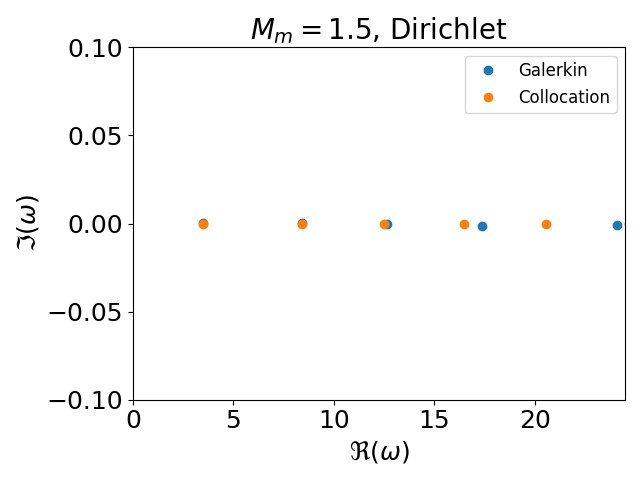
\includegraphics[width=0.7\linewidth]{figures/supersonic-drichlet.png}
	\caption{First 5 eigenmodes are shown, they are stable. Two methods agree well on the first 3 eigenmodes, and starts to deviate from each other after that.}
	\label{fig:supersonic-dirichlet}
\end{figure}

\subsubsection*{Fixed-Open Boundary}
All modes are unstable.
\begin{figure} [H]
	\centering
	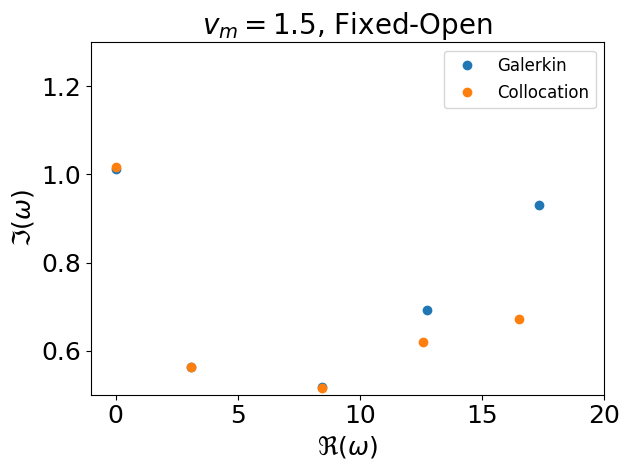
\includegraphics[width=0.7\linewidth]{figures/supersonic-fixed-open.png}
	\caption{Showing the first 5 filtered eigenmodes, they are unstable. Two methods agree well on the first 3 modes, and start to have significant difference after that.}
	\label{fig:supersonic-fixed-open}
\end{figure}


\section{Accelerating Case}
Starting from the singular point, we shoot the solution to the left boundary. We find the set of eigenvalues such that $\tilde{v}(-1)=0$. With these eigenvalues, we can extend the solution to the supersonic region $(0,1]$. The first few eigenmodes are drawn in Fig.~\ref{fig:results-accelerating-v}.
\begin{figure} [H]
	\centering
	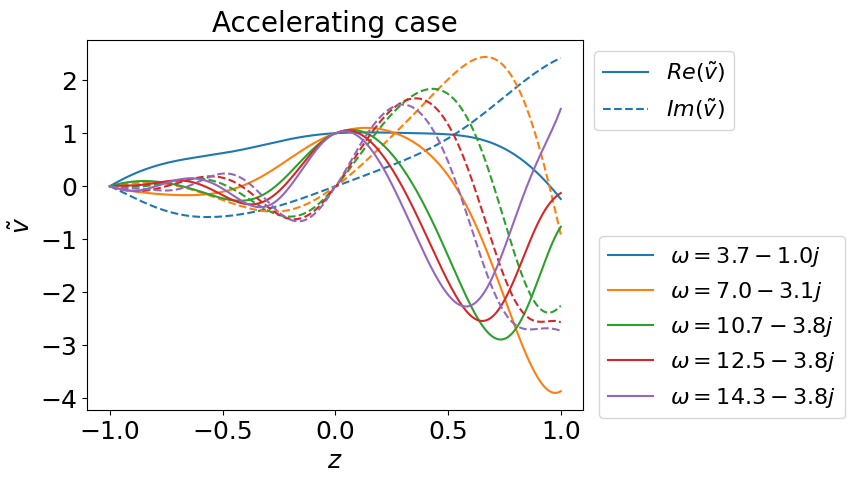
\includegraphics[width=0.7\linewidth]{figures/results-accelerating-v}
	\caption{Showing the first 5 eigenmodes, they are stable.}
	\label{fig:results-accelerating-v}
\end{figure}
